\cleardoublepage

\section{于汉的研究}

于汉在他的文章《Weak tangent and level set of Takagi functions》一文中介绍了Takagi函数,并证明了在特定参数下Takagi函数的一些性质。


\subsection{Takagi函数的水平集及其Hausdorff维数}

\begin{definition}[Takagi 函数]
      以下函数称为Takagi函数
      $$
      T_{a,b}(x)=\sum_{n=0}^\infty a^nT(b^nx),
      $$
      其中,$a<1,b>1,ab\ge1$,且$T:\mathbb{R}\rightarrow\mathbb{R}$是周期为$1$ 的帐篷函数,其在区间$[0,1]$上的定义为
      $$
      T(x)=
      \begin{cases}
            x~~~~~~,x\in[0,\frac{1}{2}],\\
            1-x,x\in[\frac{1}{2},1].
      \end{cases}
      $$
\end{definition}



\begin{definition}[水平集]
    设函数$f:[0,1]\rightarrow\mathbb{R}$,$\forall y \in\mathbb{R}$,定义函数$f$的水平集为,
    $$
        L(y)=\{x\in[0,1]:f(x)=y\}\times\{y\}.
    $$
\end{definition}

\begin{definition}[Littlewood多项式]
      称所有系数的取值都在$\{1,-1\}$中的$k$阶多项式为$k$阶Littlewood多项式,即
      $$
      \sum_{n=0}^k\epsilon_nx^n=0,
      $$
      其中,$\epsilon_n\in\{1,-1\},n=0,1,\cdots,k$。
\end{definition}

下面我们给出几个常见的维数的定义,
\begin{itemize}

      \item 盒维数

      集合$F$的盒维数定义为
      $$
      \mathrm{\dim_B}F=\lim\limits_{r\rightarrow0}\frac{\log N_r(F)}{-\log r}.
      $$

      \item Hausdorff维数

      集合$F$的Hausdorff维数定义为
      $$
      \mathrm{\dim_H}F=\inf\Big\{s:\forall\delta>0,\exists\{U_i\}_{i=1}^\infty,\mbox{使得}\bigcup_{i=1}^\infty U_i\supset F,\mbox{且}\sum_{i=1}^\infty (\mathrm{diam}~U_i)^s<\delta\Big\}.
      $$

      \item Assouad维数

      集合$F$的Assouad维数定义为
      $$
      \mathrm{\dim_A}F=\inf\Big\{s:(\exists C>0)(\forall R>0)\big(\forall r\in(0,R)\big)(\forall x\in F),N_r\big(B(x,R)\cap F\big)\le C\Big(\frac{R}{r}\Big)^s\Big\}.
      $$

\end{itemize}



于汉的第一个结论为,参数$a,b$满足$0<a<1,b>1,2|b,ab\ge1,ab$为$k-1$阶Littlewood多项式的根的Takagi函数具有一个较大的水平集,这个水平集的Hausdorff维数不小于$\frac{1}{k}$。

\begin{proof}
    由条件,$\exists\epsilon_n\in\{1,-1\},n=0,1,\cdots,k-1$,使得$ab$为以下$k-1$阶Littlewood多项式的根,
    $$
        \sum_{n=0}^{k-1}\epsilon_n(ab)^n=0.
    $$

    取$T_{a,b}(x)$的前$k$项部分和,记为$F_1(x)$,
    $$
        F_1(x)=\sum_{n=0}^{k-1}a^nT(b^nx),
    $$
    显然,对任意的正整数$m$,$x=mb^{-k}$为$F_1(x)$的不可导点。

    我们有
    $$
        \begin{aligned}
            F_1(1-x) & =\sum_{n=0}^{k-1}a^nT(b^n(1-x))=\sum_{n=0}^{k-1}a^nT(b^n-b^nx) \\
                   & =\sum_{n=0}^{k-1}a^nT(1-b^nx)=\sum_{n=0}^{k-1}a^nT(b^nx)=F_1(x).
        \end{aligned}
    $$
    故$F_1(x)$关于直线$x=\frac{1}{2}$对称。

    对$F_1(x)$求导,可得
    $$
        F_1'(x)=\sum_{n=0}^{k-1}(ab)^nT'(b^nx).
    $$

    记$\epsilon_n(x)=T'(b^nx)$,则
    $$
        F_1'(x)=\sum_{n=0}^{k-1}\epsilon_n(x)(ab)^n,
    $$
    其中,$\epsilon_n(x)\in\{1,-1\}$,其取值取决于$x$以$b$为基数的展开式。若假设$x$以$b$为基数的展开式为
    $$
        x=0.x_1x_2\cdots
    $$
    由于$T(x)$周期为$1$,其导数的周期也为$1$,故有
    $$
        T'(b^nx)=T'(x_1x_2\cdots x_n.x_{n+1}\cdots x_k\cdots)=T'(0.x_{n+1}\cdots x_k\cdots),n=0,1,\cdots,k-1.
    $$
    则有
    $$
        \epsilon_n(x)=
        \begin{cases}
            1,x_{n+1}\in[0,\frac{b}{2}),\\
            -1,x_{n+1}\in[\frac{b}{2},b),
        \end{cases},n=0,1,\cdots,k-1.
    $$

    因此,我们可以找到$b_1,b_2,\cdots,b_k$并令$x_i=b_i,i=1,2,\cdots,k$,即可使$\epsilon_n(x)=\epsilon_n,n=0,1,\cdots,k-1$,从而有
    $$
        F_1'(x)=\sum_{n=0}^{k-1}\epsilon_n(x)(ab)^n=\sum_{n=0}^{k-1}\epsilon_n(ab)^n=0.
    $$

    此时,我们仅改变$b_k$的取值,若$b_k<\frac{b}{2}$,则令其取遍$[0,\frac{b}{2})$,反之则取遍$[\frac{b}{2},b)$,则我们得到了$\frac{b}{2}$个长度为$\frac{1}{b^k}$的区间,这些区间是被仅挖去了点$x=mb^{-k},m\in\mathbb{Z}^+$的连续区间,故在这些区间上,我们得到$F_1'(x)=0$,存在$a_1\in\mathbb{R}$,使得$F_1(x)=a_1$。

    因为$\underset{n=0}{\overset{k-1}{\sum}}\epsilon_n(ab)^n=0$,则有$\underset{n=0}{\overset{k-1}{\sum}}(-\epsilon_n)(ab)^n=0$。
    又因为$F_1(x)$关于直线$x=\frac{1}{2}$对称,故我们可以找到与上述$\frac{b}{2}$个区间一一对称的$\frac{b}{2}$个区间,在这些区间上$\epsilon_n(x)=-\epsilon_n$,且有$F_1(x)=a_1$。

    至此,我们找到了$b$个长度为$\frac{1}{b^k}$的区间,将这些区间内所有点的集合记为$I_1$,由此,我们可以得到一个$F_1(x)$的水平集$L(a_1)=\{x:x\in I_1\}\times\{a_1\}$。

    取Takagi函数的第二个$k$项部分和,记为$F_2(x)$,即
    $$
        F_2(x)=\sum_{n=k}^{2k-1}a^nT(b^nx)=\sum_{n=0}^{k-1}a^k\cdot a^nT(b^n\cdot b^kx)=a^kF_1(b^kx),
    $$
    不难看出,存在与$b_1,\cdots,b_k$取法相同,但取值可能不同的$b_{k+1},b_{k+2},\cdots,b_{2k}$并令$x_i=b_i,i=k+1,\cdots,2k$,即可使$F_2'(x)=(ab)^kF_1'(b^kx)=0$,即存在$a_2\in\mathbb{R}$,使得$F_2(x)=a_2$。

    同上,我们令$b_{2k}$取遍它所在的区间的值,可得$\frac{b}{2}$个区间,并加上与这些区间对称的区间,这样可得$b$个区间。

    再将前$k$个$x_i$的取值继承下来,这样,我们就得到了$b^2$个长度为$\frac{1}{b^{2k}}$的区间,将这些区间内所有点的集合记为$I_2$,这可以构成$F_1(x)+F_2(x)$的一个水平集$L(a_1+a_2)=\{x:x\in I_2\}\times\{a_1+a_2\}$。

    不断重复上述过程,不难得到,在第$m$次迭代时,我们可以构造出集合$I_m$,这个集合由$b^m$个长度为$\frac{1}{b^{mk}}$的区间内的所有点构成,
    使得$\forall x\in I_m$,有
    $$T'(b^nx)=\epsilon_{N(n)},orT'(b^nx)=-\epsilon_{N(n)},n=1,2,\cdots,mk,$$
    其中$N(n)=n(\mathrm{mod}~k)$,且有$\forall 0\le t<m$,
    $$
            \frac{T'(b^{tk+1}x)}{\epsilon_1}=\frac{T'(b^{tk+2}x)}{\epsilon_2}=\cdots=\frac{T'(b^{(t+1)k}x)}{\epsilon_k}.
    $$

    这样,我们得到了$b^m$个长度为$b^{-mk}$的区间,在这些区间上,$\exists y_m= \sum_{n=1}^ma_m\in\mathrm{R}$,使得,$\sum_{n=1}^mF_n(x)=y_m$,由此,我们可以构造水平集

    $$
        L(y_m)=\{x:x\in I_m\}\times\{y_m\}.
    $$

    而这个水平集$L(y_m)$的Hausdorff维数$s_m$满足
    $$
        \exists \{U_i\}_{i=1}^{b^m},\forall i,\mathrm{diam}U_i=\frac{1}{b^{mk}},\mbox{使得},\bigcup_{i=1}^{b^m}U_i\supset L_m(y_m),
    $$
   且$\forall \delta>0$,
    $$
        \sum_{i=1}^{b^m}\big(\mathrm{diam}U_i\big)^{s_m}<\delta,\Rightarrow
        b^{m}\cdot b^{-mks_m}<\delta.
    $$

    当我们令$m\rightarrow\infty$时,我们就能得到Takagi函数的水平集$L(y)$,则其Hausdorff维数$s=\lim\limits_{m\rightarrow\infty}s_m$满足$\forall\delta>0$,
    $$
        \lim\limits_{m\rightarrow\infty}\big(b^{1-ks_m}\big)^{m}<\delta,
    $$
    即,
    $$
        \lim\limits_{m\rightarrow\infty}b^{1-ks_m}<1\Rightarrow \lim\limits_{m\rightarrow\infty}s_m>\frac{1}{k}\Rightarrow s>\frac{1}{k}.
    $$

\end{proof}

\subsection{Takagi函数图像的Assouad维数}

记函数$f:[0,1]\rightarrow\mathbb{R}$的图像为$\Gamma_f$,即
$$
      \Gamma_f=\big\{(x,y):x\in[0,1],y=f(x)\big\}.
$$


\begin{lemma}\cite{1}
      假设$f:[0,1]\rightarrow\mathbb{R}$是Lipschitz常数为$M>0$的Lipschitz连续函数,$g:[0,1]\rightarrow\mathbb{R}$是连续函数,则$\forall 0<r<R<1$,当$\frac{R}{r}\in\mathbb{Z}^+$时,有以下不等式:
      $$
            \sup\limits_{a\in[0,1]\times\mathbb{R}} N\big(S(a,\frac{R}{2})\cap \Gamma_{f+g},r\big)\\
            \ge \frac{1}{M+2}\sup\limits_{a\in[0,1]\times\mathbb{R}}N\big(S(a,\frac{R}{2})\cap\Gamma_g,r\big)-\frac{M+2}{\lfloor M\rfloor +2}\cdot \frac{R}{r}.
      $$
\end{lemma}

\begin{lemma}\cite{1}
      若$1<\beta<2$,则有,$\forall k\in\mathbb{Z}^+$,存在一个序列$\{\epsilon_n\}_{n=0}^k\in\{-1,1\}$,使得,
      $$
      \Big|\sum_{n=0}^k\epsilon_n\beta^n\Big|<\frac{1}{\beta-1}.
      $$
\end{lemma}

\begin{proof}
      我们构造$f_1(x)=\beta x+1,f_{-1}(x)=\beta x -1$,则我们可得:
      $$
      \sum_{n=0}^k\epsilon_n\beta^n=\epsilon_0+\beta\cdot\Big(\epsilon_1+\beta\cdot\big(\cdots+\beta\cdot(\epsilon_k+\beta\cdot0)\big)\Big)=f_{\epsilon_0}\circ f_{\epsilon_1}\circ \cdots f_{\epsilon_k}(0).
      $$
      此时,我们可以绘制以下图像,
      \begin{figure}[H]
            \centering
            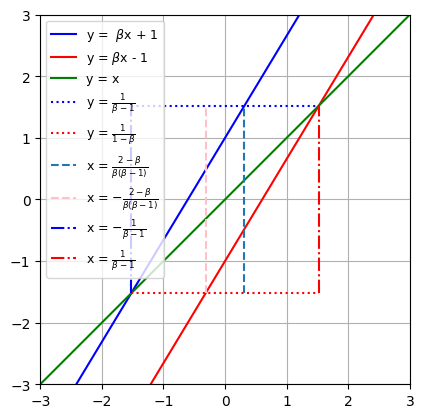
\includegraphics[scale=0.5]{Conclusion2.png}
            \caption{不动点及边界图像}
            \label{fig:C1onclusion2}
      \end{figure}

      由图像可以看出,当$x\in\big(-\frac{1}{\beta-1},\frac{2-\beta}{\beta(\beta-1)}\big)$,有$f_1(x)\in\big(-\frac{1}{\beta-1},\frac{1}{\beta-1}\big)$,而当$x\in\big(-\frac{2-\beta}{\beta(\beta-1)},\frac{1}{\beta-1}\big)$,有$f_{-1}(x)\in\big(-\frac{1}{\beta-1},\frac{1}{\beta-1}\big)$。

      又有$\big(-\frac{1}{\beta-1},\frac{2-\beta}{\beta(\beta-1)}\big)\cup\big(-\frac{2-\beta}{\beta(\beta-1)},\frac{1}{\beta-1}\big)=\big(-\frac{1}{\beta-1},\frac{1}{\beta-1}\big)$,故可得
      $$
      \forall x\in\big(-\frac{1}{\beta-1},\frac{1}{\beta-1}\big), \exists i\in\{-1,1\},\mbox{ 使得}f_i(x)\in(-\frac{1}{\beta-1},\frac{1}{\beta-1}).
      $$

      由此,因为$f_{\epsilon_k}(0)=1\in(-\frac{1}{\beta-1},\frac{1}{\beta-1})$,故有,存在一个序列$\{\epsilon_n\}_{n=0}^{k}\in\{-1,1\}$,使得
      $$
      \Big|\sum_{n=0}^k\epsilon_n\beta^n\Big|<\frac{1}{\beta-1}.
      $$
\end{proof}

\begin{lemma}\cite{1}
      假设$T_{a,b}(x):\mathbb{R}\rightarrow\mathbb{R}$为以下形式的函数:
      $$
      T_{a,b}(x)=\sum_{n=0}^\infty a^nT(b^nx),
      $$
      其中$T(x):\mathbb{R}\rightarrow\mathbb{R}$是周期为$1$的$C^1$连续函数,且$a>0,b>0,ab>1$。若以下两个条件成立:
      \begin{enumerate}
            \item 存在一个常数$C_1>0$,使得,对任意的正整数$M>0$,存在一个正整数$k$使得$J_k=(\frac{k}{b^{M+1}},\frac{k+1}{b^{M+1}})$,且$\forall x_1,x_2\in J_k$,以下不等式成立
            $$
            \Big|\sum_{n=0}^Ma^nT(b^nx_1)-\sum_{n=0}^Ma^nT(b^nx_2)\Big|<C_1|x_1-x_2|.
            $$
            \item 存在一个水平集$L\subset[0,1]$,其下盒维数不小于$D$,即
            $$
            \exists y\in\mathbb{R},\underline{\mathrm{\dim_B}}L(y)=\underline{\mathrm{\dim_B}}\{x\in[0,1]:T_{a,b}(x)=y\}\ge D.
            $$
      \end{enumerate}

      则有以下结论
      $$
      \mathrm{\dim_A\Gamma_{T_{a,b}}}\ge D+1.
      $$

\end{lemma}

\begin{proof}
      由条件,对任意的正整数$M>0$,可以找到一个整数$k$和$x_0=\frac{k}{b^{M+1}}$使得
      $$J_k=(x_0,x_0+\frac{1}{b^{M+1}})\subset[0,1],$$
      在这个区间内,$\exists C_1>0,\forall x_1,x_2\in J_k$,
            $$
                  \bigg|\sum_{n=0}^{M}a^nT(b^nx_1)-\sum_{n=0}^{M}a^nT(b^nx_2)\bigg|<C_1|x_1-x_2|.
            $$

            故可以将原函数写为
            $$
                  T_{a,b}(x)=\sum_{n=0}^{\infty}a^nT(b^nx)=\sum_{n=0}^{M}a^nT(b^nx)+\sum_{n=M+1}^{\infty}a^nT(b^nx)=F_M(x)+G_M(x),
            $$
            其中$F_M(x),G_M(x)$分别是第三个表达式中的前后两个部分和。

            不难看出,$\Gamma_{G_M}$是$\Gamma_{T_{a,b}}$的一个压缩版本,并满足以下关系
            $$
                  X_M(\Gamma_{T_{a,b}})=\Gamma_{G_M},
            $$
            其中$X_M:\mathbb{R}^2\rightarrow\mathbb{R}^2$为线性变换,定义如下
            $$
                  X_M(x,y)=\big(\frac{x}{b^{M+1}},a^{M+1}y\big).
            $$

            当$M$足够大时,这个线性变换会将图像压缩到非常细的矩形中,我们集中到下面这个矩形中
            $$
                  S=\big(x_0,x_0+\frac{1}{b^{M+1}}\big)\times\mathbb{R},
            $$
            则这个矩形中的图像$\Gamma_{G_M}$是$[0,1]$上的图像$\Gamma_{T_{a,b}}$的一个压缩版本。

            对$\Gamma_{G_M}$估计其Assouad维数,可以先用边长为$b^{-(M+1)}$的正方形进行覆盖,再用边长为$r$的正方形覆盖,其中,$r$的具体数值会在后面确定。通过$X_M$的逆映射,对$\Gamma_{G_M}$先用边长为$b^{-(M+1)}$的矩形进行覆盖,再用边长为$r$的矩形覆盖,相当于对$\Gamma_{T_{a,b}}$先用$1\times(ab)^{-(M+1)}$的矩形进行覆盖,再用$rb^{M+1}\times ra^{-(M+1)}$的矩形覆盖。

            由条件,$\exists y'\in\mathbb{R}$,使得$\mathrm{\dim_BL(y')}\ge D$,其中$L(y')=\{x\in[0,1]:T_{a,b}(x)=y'\}\times\{y'\}$。

            对$L(y')$,在包含$L(y')$的$1\times(ab)^{-(M+1)}$的矩形内进行盒计数。不妨设$\forall (x,y')\in L(y')$,我们令这些点落在矩形与$x$轴平行的平分线上。

            若$M$足够大,我们需要至少$(ab)^{(D-\delta)(M+1)}$个边长为$(ab)^{-(M+1)}$的正方形来覆盖这个$1\times (ab)^{-(M+1)}$的矩形,因为覆盖$L(y')$就需要这么多个正方形。而对每一个正方形,我们都需要
            $\frac{1/(ab)^{M+1}}{r/a^{M+1}}=b^{-(M+1)}/r$
            个$rb^{M+1}\times ra^{-(M+1)}$的矩形来覆盖。

            现在,我们可得
            $$
                  r = \frac{1}{(ab^2)^{M+1}}=\big(\frac{1}{(ab)^{M+1}}\big)^{\frac{\ln ab^2}{\ln ab}}=\big(\frac{1}{(ab)^{M+1}}\big)^{\frac{B}{B-1}}=\big(\frac{1}{b^{M+1}}\big)^B.
            $$
            其中$B=2+\ln a/\ln b$是$\Gamma_{T_{a,b}}$的上盒维数。记$R=b^{-(M+1)},r=R^{\frac{1}{\theta}}$,其中$\theta=1/B$,则当$M$充分大时,有
            $$
                  \sup\limits_{a\in\mathbb{R}^2}N(S(a,\frac{R}{2})\cap\Gamma_{G_M},R^{\frac{1}{\theta}})\ge\big(\frac{1}{ab}\big)^{-(D-\delta)(M+1)}=(\frac{R}{r})^{1+D-\delta}.
            $$

            由引理1,我们可得
            $$
                  \begin{aligned}
                        &\sup\limits_{a\in[x_0,x_0+\frac{1}{b^{M+1}}]\times\mathbb{R}}N\big(S(a,\frac{R}{2})\cap\Gamma_{T_{a,b}},r\big)\\
                              &\ge C\sup\limits_{a\in[x_0,x_0+\frac{1}{b^{M+1}}]\times\mathbb{R}}N\big(S(a,\frac{R}{2})\cap\Gamma_{G_M},r\big)-C\frac{R}{r}\\
                              &\ge C\big(\frac{R}{r}\big)^{1+D-\delta}-C\frac{R}{r}.
                  \end{aligned}
            $$

            由Assouad维数的定义可知
            $$
                  \mathrm{\dim_A}\Gamma_{T_{a,b}}\ge1+D.
            $$
\end{proof}

下证Takagi函数$T_{a,b}(x)$满足引理3中的条件1。


\begin{proof}
      假设$a<1,2|b,1<ab<2$,则对任意的$M>0$,我们考虑以下区间$J_M(l)=\big[\frac{l}{b^M},\frac{l+1}{b^M}\big],l\in\mathbb{Z}$,若$b\ge3$,有
      $$
            \frac{1}{b^M}\ge3\times\frac{1}{b^{M+1}},
      $$
      这说明了$J_M(l)$至少包含两个完整的$J_{M+1}$的区间,我们记为$J_{M+1}(t),J_{M+1}(t+1)$,这个结论在$b=2$时也成立,故对$2|b$的情况都成立。

      不难得,
      $$
      T'(b^{M-1}x)=\begin{cases}
            1,t\mbox{为奇数}\\
            -1,t\mbox{为偶数}.
      \end{cases}
      $$

      我们记$\beta_n=T'(b^nx),n=0,1,\cdots,M$。

      我们定义
      $$
      D_M(x)=\sum_{n=0}^Ma^n(T(b^nx))'=\sum_{n=0}^M(ab)^nT'(b^nx)=\sum_{n=0}^M\beta_n(ab)^n.
      $$

      由引理2可知,我们可以找到$\eta_n\in\{1,-1\},n=0,1,\cdots,M$,使得$D_M(x)$有界,即$\forall M>0$我们可以找到一列区间$J_M(t_M)\subset J_{M-1}(t_{M-1})\subset\cdots\subset J_1(t_1)$,使得$\beta_n=\eta_n,n=0,1,\cdots,M$,故有$\forall M>0,\exists t\in\mathbb{Z},\exists C_1\in\mathbb{R}$使得$\forall x_1,x_2\in \big[\frac{t}{b^M},\frac{t+1}{b^M}\big]$,有

      $$
      \Big|\sum_{n=0}^Ma^nh(b^nx_1)-\sum_{n=0}^Ma^nh(b^nx_2)\Big|<C_1|x_1-x_2|.
      $$
\end{proof}

此时,我们已知$T_a.b(x)$满足引理3中的条件1,且根据第一个结论,$\exists y\in\mathbb{R}$使得$T_{a,b}(x)$存在一个水平集$L(y)$,其Hausdorff维数不小于$1/k$。
故由引理3,可知,当$0<a<1,2|b,1<ab<2$时,有
$$
      \mathrm{\dim_A\Gamma_{T_{a,b}}}\ge\mathrm{\dim_B}L(y)+1\ge\mathrm{\dim_H}L(y)+1\ge1+\frac{1}{k}.
$$

以上便是于汉在文中的两个重要的结论,接下来,我将把这两个结论推广到一类广义Takagi函数上。


\newpage

\section{一类广义Takagi函数及其性质}

\subsection{由可分割折线函数产生的广义Takagi函数的定义}

设$h(x)$是周期为1,且关于直线$x=\frac{1}{2}$对称,并且在$[0,1]$区间上为分段线性的连续函数,即$\exists0=x_0<x_1<\cdots<x_N=1$,使得$\forall 1\le i\le N$,$h(x)$在$[x_{i-1},x_i]$上为线性函数。

同时,根据$h(x)$的不可导点对$[0,1]$区间进行划分,可以得到$\mathbb{I}=\{I_1,I_2,\cdots,I_N\}$,其中$I_1,\cdots,I_N$从左到右排列。

若$N\ge2,\forall i,j\in\{1,2,\cdots,N\},\frac{|I_i|}{|I_j|}\in\mathbb{Q}$,则称$h(x)$为可分割折线函数。



\subsection{广义Takagi函数的水平集及其Hausdorff维数}

假设$h(x)$为可分割函数,其在$[0,1]$上按不可导点被分割的区间族为$\mathbb{I}=\{I_1,I_2,\cdots,I_N\}$,其中$I_1,\cdots,I_N$从左到右排列。并设$h(x)$在区间$I_i$上的导数值为$K_i$。设$\mathbb{I}$中$h(x)$的导数不为$0$的区间中,区间长度最大的为$I_{J^*}$,记其上的导数为$K_{J^*}$,由于$h(x)$关于$x=\frac{1}{2}$对称,故$|I_{N+1-J^*}|=|I_{J^*}|$且$I_{N+1-J^*} $上的导数为$-K_{J^*}$。

我们定义广义Takagi函数$H_{a,b}(x)$如下,
$$
      H_{a,b}(x)=\sum_{n=0}^\infty a^nh(b^nx),
$$
其中$a,b$满足$0<a<1,b>1$,$ab$为$k-1$阶Littlewood多项式的根,且$n(\mathbb{I})|b$,则对函数$H_{a,b}(x)$,存在$y\in\mathbb{R}$,使得
$$
      \mathrm{dim_H}L(y)\ge\frac{1}{k}\Big(1+\log_b2|I_{J^*}|\Big).
$$

\begin{proof}
由条件,$\exists \epsilon_n\in\{1,-1\},n=0,1,\cdots,k-1$,使得$ab$为以下$k-1$阶Littlewood多项式的根
$$
      \sum_{n=0}^{k-1}\epsilon_n(ab)^n=0.
$$
我们取$H_{a,b}(x)$的前$k$项部分和,记为$H_1(x)$,
$$
      H_1(x)=\sum_{n=0}^{k-1}a^nh(b^nx),
$$
我们有
$$
    \begin{aligned}
        H_1(1-x)&=\sum_{n=0}^{k-1}a^nh(b^n(1-x))=\sum_{n=0}^{k-1}a^nh(b^n-b^nx)\\
                &=\sum_{n=0}^{k-1}a^nh(1-b^nx)=\sum_{n=0}^{k-1}a^nh(b^nx)=H_1(x).
    \end{aligned}
$$
故$H_1(x)$关于直线$x=\frac{1}{2}$对称。

对其求导,可得
$$
      H_1'(x)=\sum_{n=0}^{k-1}(ab)^nh'(b^nx),
$$
我们记$\epsilon_n(x)=h'(b^nx)$,则
$$
      H_1'(x)=\sum_{n=0}^{k-1}\epsilon_n(x)(ab)^n,
$$
若我们可令$\epsilon_n(x)=\epsilon_n$,我们可得$H_1'(x)=0$。

$\forall x\in[0,1]$将$x$以$b$为基数展开,并假设其展开形式为$x=0.x_1x_2\cdots x_n\cdots$。

$\forall b_1,b_2,\cdots,b_k\in\{0,1,2\cdots,b-1\}$,定义
$$
      I^1(b_1b_2\cdots b_k)=\{x:x\mbox{展开式小数点后的第}1\mbox{项到第}k\mbox{项为}b_1b_2\cdots b_k\}.
$$

根据$b_n,n=1,2,\cdots,k$的取值,我们一共可以生成$b^k$个连续的,长度为$\frac{1}{b^k}$的上述区间。由于$n(\mathbb{I})|b$,故有$\frac{|I_i|}{1/b^k}=|I_i|\cdot b^k=\frac{n(I_i)}{n(\mathbb{I})}\cdot b^k\in\mathbb{Z},i=1,2,\cdots,N$。

我们知道,对$x\in I^1(b_1b_2\cdots b_k)$,有
$$
      x=0.b_1b_2\cdots b_kx_{k+1}x_{k+2}\cdots,
$$
$$
b^{n}x=b_1b_2\cdots b_{n}.b_{n+1}\cdots b_kx_{k+1}x_{k+2}\cdots,0\le n\le k-1.
$$

又有$h(x)$的周期为1,则其导数的周期也为1。故$\forall0\le n\le k-1$,
$$
      h'(b^nx)=h'(b_1b_2\cdots b_n.b_{n+1}\cdots b_kx_{k+1}\cdots)=h'(0.b_{n+1}\cdots b_kx_{k+1}\cdots).
$$

因此,我们可得以下结论:

$$
      \epsilon_n(x)=h'(b^nx)=h'(0.b_{n+1}\cdots b_k\cdots)=            K_j,b_{n+1}\in{\big[}\frac{b}{n(\mathbb{I})}\sum_{i=1}^{j-1}n(I_i),\frac{b}{n(\mathbb{I})}\sum_{i=1}^{j}n(I_i){\big)},j=1,2,\cdots,N.
$$

由此,我们可以找到对应的$\tilde{b}_1,\tilde{b}_2,\cdots,\tilde{b}_{k-1},\tilde{b}_k$,使得$\forall x\in I^1(\tilde{b}_1\tilde{b}_2\cdots \tilde{b}_k),\epsilon_n(x)=\epsilon_nK_{J^*},n=0,1,2,\cdots,k-1$。若给定$\tilde{b}_1,\tilde{b}_2,\cdots,\tilde{b}_{k-1}$,我们可以令$\tilde{b}_k$取遍${\big[}\frac{b}{n(\mathbb{I})}\sum_{i=0}^{J^*-1}n(I_i),\frac{b}{n(\mathbb{I})}\sum_{i=0}^{J^*}n(I_i){\big)}$
或${\big[}\frac{b}{n(\mathbb{I})}\sum_{i=0}^{N-J^*}n(I_i),\frac{b}{n(\mathbb{I})}\sum_{i=0}^{N+1-J^*}n(I_i){\big)}$,这样,我们得到了$\frac{n(I_{J^*})}{n(\mathbb{I})}b$个长度为$\frac{1}{b^k}$的区间,这些区间相互连接,仅被挖去了端点。同时,在这些区间上,我们有
$$
      H_1'(x)=\sum_{n=0}^{k-1}\epsilon_n(x)(ab)^n=\sum_{n=0}^{k-1}\epsilon_nK_{J^*}(ab)^n=K_{J^*}\sum_{n=0}^{k-1}\epsilon_n(ab)^n=0.
$$
故在这些区间上$H_1(x)$取常值,记为$y_1$。

由于$\underset{n=0}{\overset{k-1}{\sum}}\epsilon_n(ab)^n=0$,所以$\underset{n=0}{\overset{k-1}{\sum}}(-\epsilon_n)(ab)^n=0$。

由于$H_1(x)$关于$x=\frac{1}{2}$对称,我们可以找到另外的$\frac{n(I_J^*)}{n(\mathbb{I})}b$个区间,在这些区间上,$\epsilon_n(x)=-\epsilon_nK_M$,故$H'_1(x)=0,H_1(x)\equiv y_1$。由此,我们找到了$H_1(x)$的$y_1$的一个水平集,它由$\frac{2n(I_J^*)}{n(\mathbb{I})}$个长度为$\frac{1}{b^k}$的区间构成,我们将这个水平集记为$L_1$。

现取第二个$k$项部分和,记为$H_2(x)$
$$
      \begin{aligned}
            H_2(x)= \sum_{n=k}^{2k-1}a^nh(b^nx)= \sum_{n=0}^{k-1}a^{k+n}h(b^{k+n}x)= a^kH_1(b^kx).
      \end{aligned}
$$

因此,我们可以构造如下区间:
$$
      I^2(b_{k+1}b_{b+2}\cdots b_{2k})=\{x:x\mbox{展开式小数点后的第}k+1\mbox{项到第}2k\mbox{项为}b_{k+1}b_{k+1}\cdots b_{2k}\}.
$$

考虑$I^1\cap I^2$,这是将原先长为$\frac{1}{b^k}$的区间再进行$b^k$等分,即分成长为$\frac{1}{b^{2k}}$的区间。

现对$b_{k+1}\cdots b_{2k}$按与上述相同的取法,这样可以在第一轮选出的$\frac{2n(I_J^*)}{n(\mathbb{I})}b$个区间内,每个区间内可以再找出$\frac{2n(I_J^*)}{n(\mathbb{I})}b$个小区间。故共可得$\big[\frac{2n(I_J^*)}{n(\mathbb{I})}b\big]^2$个长度为$\frac{1}{b^{2k}}$的区间,在这些区间上,同时满足$H'_1(x)=0,H'_2(x)=0$,且由于周期性与对称性,在这些区间上,$H_1(x)$取常值$y_1,H_2(x)$取常值,记为$y_2$,并将此水平集记为$L_2$。

按此方法迭代,我们可以在第$m$次迭代时,我们可得$\big[\frac{2n(I_J^*)}{n(\mathbb{I})}b\big]^m$个长度为$\frac{1}{b^{mk}}$的区间构成的一个$\sum_{t=1}^mH_t(x)$的水平集,我们将这个水平集记为$L_m$,对这个集合进行Hausdorff维数的计算时,我们可以取$\big[\frac{2n(I_J^*)}{n(\mathbb{I})}b\big]^m$个直径为$\frac{1}{b^{mk}}$的小集合,这样的集合恰好可以覆盖$L_m$。

由此,我们可以得出结论,$H_{a,b}(x)=\sum_{n=0}^\infty a^nh(b^nx)$具有一个水平集$L=\bigcap_{t=1}^\infty L_t$,其中$y=\sum_{t=1}^\infty y_t$。

则$\forall \delta>0$,其Hausdorff维数$s$有:

$$
      \lim_{m\rightarrow\infty}\Big[\frac{2n(I_J^*)}{n(\mathbb{I})}b\Big]^m*\Big[\frac{1}{b^{mk}}\Big]^s<\delta.
$$

即
$$
      \lim_{m\rightarrow\infty}\Big[\frac{2n(I_J^*)}{n(\mathbb{I})}b*\frac{1}{b^{ks}}\Big]^m<\delta.
$$

即
$$
      \frac{2n(I_J^*)}{n(\mathbb{I})}b^{1-ks}<1.
$$

从而有
$$
      1-ks<\log_b\frac{n(\mathbb{I})}{2n(I_J^*)}.
$$

又有,$\frac{n(I_J^*)}{n(\mathbb{I})}=|I_J^*|$,我们可得
$$
      s>\frac{1}{k}\Big(1-\log_b\frac{n(\mathbb{I})}{2n(I_J^*)}\Big)=\frac{1}{k}\Big(1+\log_b2|I_J^*|\Big).
$$

\end{proof}

\subsection{广义Takagi函数图像的Assouad维数}

假设$H_{a,b}(x)=\sum_{n=0}^\infty a^nh(b^nx)$,其中$h(x)$为可分割折线函数,
$\mathbb{I}=\{I_1,I_2,\cdots,I_N\}$为$h(x)$在$[0,1]$区间上按$h(x)$的不可导点分割产生的区间族,
其中$I_1,\cdots,I_N$从左到右排列。

$I_J^*$为$h(x)$在$[0,1]$区间上的导数不为$0$的区间长度最大的区间,其上$h(x)$的导数为$K_{J^*}$。

假设$0<a<1,b>1,1<ab<2,n(\mathbb{I})|b$,且$ab$为$k-1$阶Littlewood多项式的根,则我们可得以下结论:

$$
      \mathrm{\dim_A}\Gamma_{H_{a,b}(x)}\ge1+\frac{1}{k}\Big(1+\log_b2|I_{J^*}|\Big).
$$

\begin{proof}

    先证明$H_{a,b}(x)$满足引理3中的第一个条件,即,

    若$a,b$满足,$0<a<1,b\ge2,n(\mathbb{I})|b,1<ab<2$,则有 $\exists C_1>0$,
    $\forall M>0,\exists k\in\mathbb{Z}^+$,使得$\forall x_1,x_2\in [\frac{k}{b^M},\frac{k+1}{b^M}]$,有

    $$
    \Big|\sum_{n=0}^Ma^nh(b^nx_1)-\sum_{n=0}^Ma^nh(b^nx_2)\Big|<C_1|x_1-x_2|.
    $$

    对任意的整数$M>0$,我们记第$M$级区间的第$t+1$个区间为

    $$
    O_M(t)=\big[\frac{t}{b^M},\frac{t+1}{b^M}\big],t\in\mathbb{Z}.
    $$

    由于我们取的$b$一定为整数,$I_M(t)$可被分为$b$个区间,因此,我们有以下结论

    $$
    h'(b^{M-1}x)=\begin{cases}
        K_{J^*},~~x\in O_M(t),t(\mathrm{mod}~b) \in {\big[}\frac{b}{n(\mathbb{I})}\sum_{i=0}^{J^*-1}n(I_i),\frac{b}{n(\mathbb{I})}\sum_{i=0}^{J^*}n(I_i){\big)},\\
        -K_{J^*},~~x\in O_M(t),t(\mathrm{mod}~b) \in {\big[}\frac{b}{n(\mathbb{I})}\sum_{i=0}^{N-J^*}n(I_i),\frac{b}{n(\mathbb{I})}\sum_{i=0}^{N+1-J^*}n(I_i){\big)}.
    \end{cases}
    $$

    我们记$\beta_n=\frac{1}{K_{J^*}}h'(b^nx),n=0,1,\cdots,M$。

      我们定义
      $$
      D_M(x)=\sum_{n=0}^Ma^n(h(b^nx))'=\sum_{n=0}^M(ab)^nh'(b^nx)=\sum_{n=0}^M\beta_n(ab)^n.
      $$

      由引理2可知,我们可以找到$\eta_n\in\{1,-1\},n=0,1,\cdots,M$,使得$D_M(x)$有界,即$\forall M>0$我们可以找到一列区间$O_M(t_M)\subset O_{M-1}(t_{M-1})\subset\cdots\subset O_1(t_1)$,使得$\beta_n=\eta_n,n=0,1,\cdots,M$,故有$\forall M>0,\exists t\in\mathbb{Z},\exists C_1\in\mathbb{R}$使得$\forall x_1,x_2\in \big[\frac{t}{b^M},\frac{t+1}{b^M}\big]$,有
    $$
    \Big|\sum_{n=0}^Ma^nh(b^nx_1)-\sum_{n=0}^Ma^nh(b^nx_2)\Big|<C_1|x_1-x_2|.
    $$

    由第一个结论,$H_{a,b}(x)$存在一个水平集$L$,其Hausdorff维数不小于$\frac{1}{k}\Big(1+\log_b 2|I_{J^*}|\Big)$,故有$\mathrm{\dim_B}L\ge\mathrm{\dim_H}L\ge\frac{1}{k}\Big(1+\log_b2|I_{J^*}|\Big)$。

    由此,$H_{a,b}(x)$满足引理3中的两个条件,故有
    $$
        \mathrm{\dim_A\Gamma_{H_{a,b}(x)}}\ge1+\frac{1}{k}\big(1+\log_b2|I_{J^*}|\big).
    $$
\end{proof}

\newpage
\section{总结与展望}
\subsection{研究总结}
本研究探讨了一类广义Takagi函数的水平集性质,旨在拓展和深化于汉在《Weak tangent and level sets of Takagi functions》中的研究成果。通过构建数学模型、运用分形几何学中的维数理论以及拓扑学的相关理论和方法,我们对这类分形函数的水平集性质进行了系统分析。研究的主要内容包括:

\begin{enumerate}
      \item 数学模型构建:详细分析了分形函数的自相似性、不可微性等基本特性,并探讨了这些特性对水平集性质的影响。
      \item 维数理论应用:运用分形几何学中的维数理论,如盒维数、Hausdorff维数和Assouad维数等,研究了水平集的维数特征。成功证明了在满足特定条件下,该类分形函数存在一个水平集,其Hausdorff维数具有明确的下界估计。
\end{enumerate}



\subsection{研究不足}
尽管本研究取得了一系列重要的理论成果,但仍存在一些不足之处:

\begin{enumerate}
      \item 精确维数计算:水平集的精确维数计算仍然是一个未解决的问题,需要进一步研究。
      \item 更广泛的参数取值范围:对于更广泛的参数取值范围内的水平集性质,需要进行更深入的分析。
      \item 拓扑结构的深入分析:水平集的拓扑结构在不同参数条件下的变化规律需要进一步深入研究。
      \item 应用探索:本研究主要集中在理论分析上,但如何将这些理论成果应用于实际问题,如图像处理、信号分析等领域,仍需进一步探索。
\end{enumerate}
\subsection{未来展望}
未来的研究工作将致力于解决上述不足,并进一步拓展分形函数水平集的研究内容和应用领域。具体计划如下:

\begin{enumerate}
      \item 精确维数计算:继续探索分形函数水平集的精确维数计算方法,发展和完善分形几何学中的维数理论。
      \item 更广泛的参数取值范围:研究更广泛的参数取值范围内的水平集性质,揭示分形函数在不同条件下的行为规律。
      \item 拓扑结构分析:深入研究水平集的拓扑结构,探索其在不同参数条件下的变化规律,为相关领域的研究提供新的视角和方法。
      \item 实际应用探索:探索分形函数水平集在图像处理、信号分析等领域的潜在应用价值,开发基于分形函数水平集的高效算法和模型,推动相关领域的研究和实践。
\end{enumerate}





总之,本研究不仅丰富了分形函数水平集的理论研究内容,还为分形几何学的发展提供了新的理论支持和研究思路。未来的研究将继续深化对分形函数水平集的理解,拓展其应用领域,为分形几何学的发展做出更多贡献。


\nocite{1}
\nocite{2}
\nocite{3}
\nocite{4}
\nocite{5}
\nocite{6}
\nocite{7}
\nocite{8}
\nocite{9}
\nocite{10}
